\documentclass[aspectratio=169,xcolor=dvipsnames,10pt]{beamer}
\usetheme{SimpleDarkBlue}
\usepackage[utf8]{inputenc}
\usepackage[english]{babel}
\usepackage{helvet}
\renewcommand{\familydefault}{\sfdefault}
\usepackage{graphicx}
\usepackage{booktabs}
\usepackage{ragged2e}
\usepackage{amsmath,amssymb,amsfonts}
\usepackage{tikz}
\usetikzlibrary{arrows.meta,positioning,fit,calc,shapes.geometric,3d}
\usepackage{bm}
\usepackage{listings}
\usepackage{pgfplots}
\pgfplotsset{compat=1.17}

% Natbib for citations
\usepackage[numbers,sort&compress]{natbib}
\bibliographystyle{unsrtnat}

% Prevent content overflowing bottom
\setbeamertemplate{frametitle continuation}{}

% -----------------------------------------------------------------------------
% METADATA
% -----------------------------------------------------------------------------
\title{FFT-Based Crystal Plasticity for\\[4pt]Large Polycrystalline Systems}
\subtitle{Physical Model\;\textbullet\;Mathematical Formulation\;\textbullet\;Numerical Implementation}
\author{Santiago Garcia Botero}
\institute{University of Texas at San Antonio}
\titlegraphic{\includegraphics[width=3cm]{utsa_logo.png}}
\date{\today}

% -----------------------------------------------------------------------------
% MACROS
% -----------------------------------------------------------------------------
\newcommand{\bvec}[1]{\mathbf{#1}}
\newcommand{\tens}[1]{\boldsymbol{#1}}
\newcommand{\grad}{\nabla}
\newcommand{\R}{\mathbb{R}}
\newcommand{\taures}{\tau^{\alpha}}
\newcommand{\gammadot}{\dot{\gamma}^{\alpha}}
\newcommand{\dif}{\mathrm{d}}
\newcommand{\avg}[1]{\langle #1 \rangle}
\newcommand{\Ebar}{\bar{\tens{\varepsilon}}}
\newcommand{\Sbar}{\bar{\tens{\sigma}}}

\lstset{
  basicstyle=\ttfamily\tiny,
  keywordstyle=\color{NavyBlue}\bfseries,
  commentstyle=\color{OliveGreen},
  stringstyle=\color{BrickRed},
  showstringspaces=false,
  breaklines=true,
  frame=single,
  language=Python,
  numbers=none
}

\begin{document}

% =============================================================================
%  TITLE
% =============================================================================
\begin{frame}
  \titlepage
\end{frame}

% =============================================================================
\begin{frame}{Outline}
  \tableofcontents
\end{frame}

% #############################################################################
%  PART I — PHYSICAL MODEL
% #############################################################################
\section{Physical Model}

% ----------- Slide 1 --------------------------------------------------------
\begin{frame}{What is Crystal Plasticity?}
\justifying

Metals are \textbf{polycrystalline} aggregates: many single crystals (grains)
bonded together, each with a different lattice orientation.

\vspace{0.6em}
\begin{columns}[T]
\begin{column}{0.52\textwidth}
\begin{itemize}
  \item \textbf{Elastic deformation:}\\
        stretching of atomic bonds (reversible).
  \item \textbf{Plastic deformation:}\\
        motion of dislocations on crystallographic
        planes (irreversible).
\end{itemize}
\end{column}
\begin{column}{0.45\textwidth}
\begin{block}{Goal}
Predict the macroscopic stress--strain response of a
polycrystal from the single-crystal constitutive law
and the grain-level microstructure.
\end{block}
\end{column}
\end{columns}
\end{frame}

% ----------- Slide 2 --------------------------------------------------------
\begin{frame}{Slip Systems in FCC Metals}
\justifying

Dislocations glide on specific \textit{slip planes}
in specific \textit{slip directions}.

\vspace{0.4em}
\begin{columns}[T]
\begin{column}{0.50\textwidth}
\textbf{Slip system $\alpha$:}
\begin{itemize}\setlength\itemsep{2pt}
  \item Plane normal: $\bvec{n}^\alpha \in \{111\}$
  \item Direction:    $\bvec{s}^\alpha \in \langle 110 \rangle$
  \item FCC $\Rightarrow$ \textbf{12 systems}
        ($4$ planes $\times$ $3$ directions)
\end{itemize}

\vspace{0.4em}
\textbf{Schmid tensor} (geometric projector):
\[
  \tens{P}^\alpha = \tfrac{1}{2}\bigl(\bvec{s}^\alpha\!\otimes\!\bvec{n}^\alpha
                  + \bvec{n}^\alpha\!\otimes\!\bvec{s}^\alpha\bigr)
\]
\end{column}
\begin{column}{0.47\textwidth}
\centering
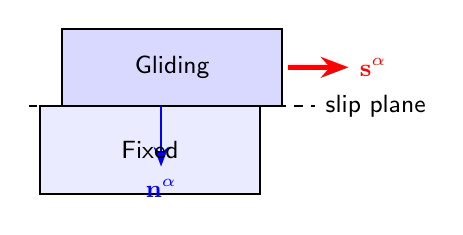
\begin{tikzpicture}[scale=0.70]
    \draw[thick, fill=blue!8] (0,0) rectangle (4,1.6);
    \draw[thick, fill=blue!15] (0.4,1.6) -- (4.4,1.6)
          -- (4.4,3.0) -- (0.4,3.0) -- cycle;
    \draw[-{Stealth[length=3.5mm]}, ultra thick, red]
          (4.5,2.3) -- (5.6,2.3) node[right,font=\small] {$\bvec{s}^\alpha$};
    \draw[dashed, thick] (-0.2,1.6) -- (5.0,1.6)
          node[right,font=\small] {slip plane};
    \draw[-{Stealth[length=2.5mm]}, thick, blue]
          (2.2,1.6) -- (2.2,0.5) node[below=1pt,font=\small] {$\bvec{n}^\alpha$};
    \node[font=\small] at (2,0.8) {Fixed};
    \node[font=\small] at (2.4,2.3) {Gliding};
\end{tikzpicture}
\end{column}
\end{columns}
\end{frame}

% ----------- Slide 3 --------------------------------------------------------
\begin{frame}{Resolved Shear Stress and Driving Force}
\justifying

The resolved shear stress on system $\alpha$ is:
\[
  \tau^\alpha = \tens{\sigma} : \tens{P}^\alpha = \sigma_{ij}\,P^\alpha_{ij}
\]

\vspace{0.2em}
\textbf{Effective driving stress} (Kocks--Argon--Ashby):
\[
  \tau_\text{drive}^\alpha = \tau^\alpha - \tau_\text{back}^\alpha,
  \qquad
  \tau_\text{eff}^\alpha
  = \bigl\langle |\tau_\text{drive}^\alpha| - S_\text{ath}^\alpha \bigr\rangle
\]

\vspace{0.3em}
\begin{itemize}\setlength\itemsep{3pt}
  \item $S_\text{ath}$: athermal (long-range) resistance ---
        grain boundaries, precipitates.
  \item $\langle \cdot \rangle$: Macaulay bracket --- no slip if
        driving stress $<$ athermal resistance.
\end{itemize}
\end{frame}

% ----------- Slide 4 --------------------------------------------------------
\begin{frame}[fragile]{Thermally Activated Flow Rule}
\justifying

Dislocation motion is \textbf{thermally activated}.
Slip rate on system $\alpha$~\cite{kocks2003}:
\[
  \dot\gamma^\alpha = \dot\gamma_\text{ref}\;
  \exp\!\Biggl[\!-\frac{\Delta G_0}{k_B T}
  \biggl(1 - \Bigl(\frac{\tau_\text{eff}^\alpha}{S_\text{th}^\alpha}\Bigr)^{\!p}
  \biggr)^{\!q}\;\Biggr]
  \;\text{sgn}(\tau_\text{drive}^\alpha)
\]

\vspace{0.2em}
\begin{columns}[T]
\begin{column}{0.45\textwidth}
\textbf{Parameters:}
\begin{itemize}\setlength\itemsep{1pt}\small
  \item $\dot\gamma_\text{ref}=10^{7}\;\text{s}^{-1}$
  \item $\Delta G_0=9.5\times10^{-19}$ J
  \item $p=0.78$, $q=1.15$
  \item $S_\text{th}$: thermal resistance
\end{itemize}
\end{column}
\begin{column}{0.52\textwidth}
\centering
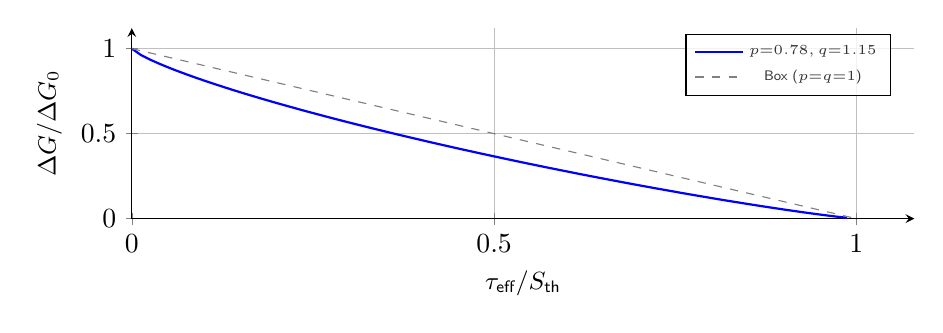
\begin{tikzpicture}
    \begin{axis}[
        width=0.95\textwidth, height=4cm,
        axis lines=left,
        xlabel={\small $\tau_\text{eff}/S_\text{th}$},
        ylabel={\small $\Delta G/\Delta G_0$},
        xtick={0,0.5,1}, ytick={0,0.5,1},
        domain=0:1, samples=80,
        xmin=0, xmax=1.08, ymin=0, ymax=1.12,
        grid=major, no markers,
        legend pos=north east,
        legend style={font=\tiny, fill opacity=0.8},
    ]
        \addplot[thick, blue] expression {(1-x^0.78)^1.15};
        \addlegendentry{$p{=}0.78,q{=}1.15$}
        \addplot[dashed, gray] expression {(1-x)};
        \addlegendentry{Box ($p{=}q{=}1$)}
    \end{axis}
\end{tikzpicture}
\end{column}
\end{columns}
\end{frame}

% ----------- Slide 5 --------------------------------------------------------
\begin{frame}{Hardening: Voce Law}
\justifying

As plastic deformation proceeds, dislocation density increases and the crystal
hardens.  \textbf{Voce law}~\cite{tome1984}:
\[
  \dot{s}^\alpha = \sum_\beta h_{\alpha\beta}\,|\dot\gamma^\beta|,
  \qquad
  h_{\alpha\beta} = q_{\alpha\beta}\;h_0\Bigl(1 - \frac{s^\beta}{s_s}\Bigr)
\]

\vspace{0.3em}
\begin{center}\small
\begin{tabular}{llr}
\toprule
\textbf{Parameter} & \textbf{Symbol} & \textbf{Cu value} \\
\midrule
Initial resistance      & $\tau_0$         & 50 MPa  \\
Saturation resistance   & $s_s$            & 200 MPa \\
Initial hardening rate  & $h_0$            & 500 MPa \\
Latent hardening ratio  & $q_\text{lat}$   & 1.4     \\
\bottomrule
\end{tabular}
\end{center}

\vspace{0.2em}
Self-hardening ($\alpha{=}\beta$): $q=1$.\quad
Latent hardening ($\alpha{\neq}\beta$): $q=1.4$.
\end{frame}

% ----------- Slide 6 --------------------------------------------------------
\begin{frame}{Polycrystalline Microstructure}
\justifying

A real metal contains $10^3$--$10^6$ grains.
We represent a \textbf{Representative Volume Element (RVE)} on a regular grid.

\vspace{0.3em}
\begin{columns}[T]
\begin{column}{0.52\textwidth}
\textbf{Voronoi tessellation} (periodic):
\begin{enumerate}\setlength\itemsep{2pt}\small
  \item Seed $N_g$ random points in $[0,1)^3$.
  \item Replicate to $3^3$ periodic images.
  \item Assign each voxel to nearest seed (KD-tree).
  \item Random Bunge Euler angles $(\varphi_1,\Phi,\varphi_2)$
        sampled with SO(3) Haar measure.
\end{enumerate}

\vspace{0.3em}
Each grain $g$ has rotation $\bvec{R}_g$ that
rotates stiffness and slip systems
into the sample frame.
\end{column}
\begin{column}{0.45\textwidth}
\centering
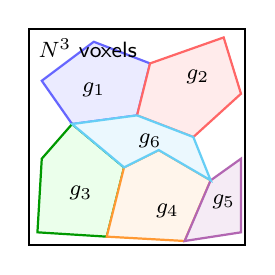
\begin{tikzpicture}[scale=0.55]
  \draw[thick] (0,0) rectangle (5,5);
  \draw[thick,blue!60,fill=blue!8]
    (0.3,3.8)--(1.5,4.7)--(2.8,4.2)--(2.5,3.0)--(1.0,2.8)--cycle;
  \draw[thick,red!60,fill=red!8]
    (2.8,4.2)--(4.5,4.8)--(4.9,3.5)--(3.8,2.5)--(2.5,3.0)--cycle;
  \draw[thick,green!60!black,fill=green!8]
    (0.2,0.3)--(1.8,0.2)--(2.2,1.8)--(1.0,2.8)--(0.3,2.0)--cycle;
  \draw[thick,orange!80,fill=orange!8]
    (1.8,0.2)--(3.6,0.1)--(4.2,1.5)--(3.0,2.2)--(2.2,1.8)--cycle;
  \draw[thick,violet!60,fill=violet!8]
    (3.6,0.1)--(4.9,0.3)--(4.9,2.0)--(4.2,1.5)--cycle;
  \draw[thick,cyan!60,fill=cyan!8]
    (2.5,3.0)--(3.8,2.5)--(4.2,1.5)--(3.0,2.2)%
    --(2.2,1.8)--(1.0,2.8)--cycle;
  \node[font=\footnotesize] at (1.5,3.6) {$g_1$};
  \node[font=\footnotesize] at (3.9,3.9) {$g_2$};
  \node[font=\footnotesize] at (1.2,1.2) {$g_3$};
  \node[font=\footnotesize] at (3.2,0.8) {$g_4$};
  \node[font=\footnotesize] at (4.5,1.0) {$g_5$};
  \node[font=\footnotesize] at (2.8,2.4) {$g_6$};
  \node[font=\footnotesize,anchor=north west] at (0,5) {$N^3$ voxels};
\end{tikzpicture}
\end{column}
\end{columns}
\end{frame}

% #############################################################################
%  PART II — MATHEMATICAL MODEL
% #############################################################################
\section{Mathematical Model}

% ----------- Slide 7 --------------------------------------------------------
\begin{frame}{Problem Statement: Equilibrium on an RVE}
\justifying

Given a periodic RVE with spatially varying stiffness $\tens{C}(\bvec{x})$
and prescribed macroscopic stress $\Sbar$ at the boundaries,
find the local fields such that:

\vspace{0.3em}
\begin{align}
  \text{Equilibrium:}\quad
    & \nabla \cdot \tens{\sigma}(\bvec{x}) = \bvec{0}
    \tag{E1} \\[3pt]
  \text{Constitutive:}\quad
    & \tens{\sigma}(\bvec{x}) = \tens{C}(\bvec{x}) : \tens{\varepsilon}(\bvec{x})
    \tag{E2} \\[3pt]
  \text{Compatibility:}\quad
    & \tens{\varepsilon} = \text{sym}(\nabla \bvec{u}),
      \;\; \bvec{u} \text{ periodic}
    \tag{E3} \\[3pt]
  \text{Average stress:}\quad
    & \avg{\tens{\sigma}} = \Sbar
    \tag{E4}
\end{align}

\vspace{0.3em}
\textbf{Key difficulty:}
$\tens{C}(\bvec{x})$ varies sharply between grains ---
anisotropic cubic elastic constants rotated by different Euler angles.

\vspace{0.2em}
\textbf{Stress control:} FFT solvers are natively strain-driven; we wrap them
in a Newton iteration on $\Ebar$ until $\avg{\tens{\sigma}} = \Sbar$.
\end{frame}

% ----------- Slide 8 --------------------------------------------------------
\begin{frame}{Lippmann--Schwinger Equation}
\justifying

Introduce a \textbf{homogeneous reference medium} $\tens{C}^0$ and
the \textbf{polarization}:
\[
  \tens{\tau}(\bvec{x})
  = \bigl[\tens{C}(\bvec{x}) - \tens{C}^0\bigr] : \tens{\varepsilon}(\bvec{x})
\]

Substituting into equilibrium and using the Green's function of $\tens{C}^0$
yields~\cite{moulinec1994,moulinec1998}:
\[
  \boxed{
    \tens{\varepsilon}(\bvec{x})
    = \Ebar - \bigl(\tens{\Gamma}^0 * \tens{\tau}\bigr)(\bvec{x})
  }
\]

\vspace{0.2em}
\begin{itemize}\setlength\itemsep{3pt}
  \item $\tens{\Gamma}^0$ is the periodic Green's operator of the reference medium.
  \item $*$ denotes spatial convolution.
  \item \textbf{Key:} in Fourier space, convolution $\to$ pointwise multiplication,
        so $\tens{\Gamma}^0$ is applied frequency by frequency.
\end{itemize}
\end{frame}

% ----------- Slide 9 --------------------------------------------------------
\begin{frame}{Green's Operator via the Acoustic Tensor}
\justifying

For an \textbf{isotropic} reference medium
$(\lambda_0, \mu_0)$,
at wave direction $\bvec{n} = \bvec{\xi}/|\bvec{\xi}|$:

\vspace{0.2em}
\begin{columns}[T]
\begin{column}{0.48\textwidth}
\textbf{Acoustic tensor:}
\[
  A_{ik} = \mu_0\,\delta_{ik} + (\lambda_0{+}\mu_0)\,n_i n_k
\]
\textbf{Analytic inverse:}
\[
  A^{-1}_{ik}
  = \frac{\delta_{ik}}{\mu_0}
  - \frac{\lambda_0{+}\mu_0}{\mu_0(\lambda_0{+}2\mu_0)}\,n_i n_k
\]
\end{column}
\begin{column}{0.48\textwidth}
\textbf{Green's operator} (Fourier space):
\begin{align*}
  b_k &= n_j\,\hat\tau_{kj}
    \\[2pt]
  \hat u_i &= A^{-1}_{ik}\,b_k
    \\[2pt]
  \hat\varepsilon'_{ij}
    &= \tfrac{1}{2}(n_i\hat u_j + n_j\hat u_i)
\end{align*}
\end{column}
\end{columns}

\vspace{0.5em}
All operations in full $(3{\times}3)$ tensor form --- no Voigt-notation
factors needed, eliminating a common source of bugs.
\end{frame}

% ----------- Slide 10 -------------------------------------------------------
\begin{frame}{Reference Medium and Stiffness Rotation}
\justifying

\begin{columns}[T]
\begin{column}{0.48\textwidth}
\textbf{Reference medium} from Voigt average:
\[
  \tens{C}^0 = \avg{\tens{C}(\bvec{x})}
\]
\[
  K_V = \frac{C^0_{11}{+}C^0_{22}{+}C^0_{33}{+}2(C^0_{12}{+}C^0_{13}{+}C^0_{23})}{9}
\]
\begin{multline*}
  \mu_V = \bigl(C^0_{11}{+}C^0_{22}{+}C^0_{33}{-}C^0_{12}{-}C^0_{13}{-}C^0_{23}\\
  +\;3(C^0_{44}{+}C^0_{55}{+}C^0_{66})\bigr) / 15
\end{multline*}
\[
  \lambda_0 = K_V - \tfrac{2}{3}\mu_V
\]
\end{column}
\begin{column}{0.48\textwidth}
\textbf{Stiffness rotation:}\\[3pt]
Each grain has the same $(C_{11},C_{12},C_{44})$
in its crystal frame but orientation $\bvec{R}_g$:
\[
  C^\text{sample}_{ijkl}
  = R_{ip}R_{jq}R_{kr}R_{ls}\,C^\text{crystal}_{pqrs}
\]

\vspace{0.3em}
\textbf{Anisotropy ratio} $A = 2C_{44}/(C_{11}{-}C_{12})$:
\vspace{0.1em}
\begin{center}\small
\begin{tabular}{lccc}
\toprule
Cu & Al & Ni & Fe \\
\midrule
3.21 & 1.22 & 2.52 & 2.36 \\
\bottomrule
\end{tabular}
\end{center}
\end{column}
\end{columns}
\end{frame}

% #############################################################################
%  PART III — NUMERICAL IMPLEMENTATION
% #############################################################################
\section{Numerical Implementation}

% ----------- Slide 11 -------------------------------------------------------
\begin{frame}{Basic Scheme (Moulinec--Suquet 1994)}
\justifying

\textbf{Fixed-point iteration} on the Lippmann--Schwinger
equation~\cite{moulinec1994,moulinec1998}:

\vspace{0.3em}
\begin{enumerate}\setlength\itemsep{2pt}\small
  \item Initialize $\tens{\varepsilon}^{(0)} = \Ebar$
  \item \textbf{Repeat} until
        $\|\Delta\tens\varepsilon\|/\|\tens\varepsilon\| < \text{tol}$:
  \begin{enumerate}\setlength\itemsep{1pt}\small
    \item[a.] $\tens{\sigma}^{(n)} = \tens{C}(\bvec{x}) : \tens{\varepsilon}^{(n)}$
    \item[b.] $\tens{\tau}^{(n)}
              = \tens{\sigma}^{(n)} - \tens{C}^0 : \tens{\varepsilon}^{(n)}$
    \item[c.] $\hat{\tens{\tau}}^{(n)} = \text{FFT}[\tens{\tau}^{(n)}]$
    \item[d.] $\hat{\tens{\varepsilon}}'
              = \tens{\Gamma}^0(\bvec{\xi})\;\hat{\tens{\tau}}^{(n)}$
              \quad {\footnotesize(pointwise, DC$\,{=}\,0$)}
    \item[e.] $\tens{\varepsilon}' = \text{IFFT}[\hat{\tens{\varepsilon}}']$
    \item[f.] $\tens{\varepsilon}^{(n+1)} = \Ebar - \tens{\varepsilon}'$
  \end{enumerate}
\end{enumerate}

\vspace{0.3em}
\textbf{Cost per iteration:} $\mathcal{O}(N^3 \log N)$ via FFT
\;(vs.\ $\mathcal{O}(N^6)$ for direct FE assembly).
\end{frame}

% ----------- Slide 12 -------------------------------------------------------
\begin{frame}{Conjugate Gradient Acceleration (Zeman 2010)}
\justifying

The basic scheme can be slow for high-contrast materials.
CG~\cite{zeman2010} solves for the \textbf{strain fluctuation}
$\tilde{\tens\varepsilon}$:
\[
  \underbrace{\bigl(\tens{I}
    + \tens{\Gamma}^0 \!\circ\! \Delta\tens{C}\bigr)}_{\tens{A}}\;
  \tilde{\tens\varepsilon}
  = -\tens{\Gamma}^0 \!\circ\! (\Delta\tens{C} : \Ebar)
  \equiv \bvec{b}
\]
where $\Delta\tens{C} = \tens{C}(\bvec{x})\!-\!\tens{C}^0$,\;
$\tens\varepsilon = \Ebar + \tilde{\tens\varepsilon}$.

\vspace{0.3em}
\begin{columns}[T]
\begin{column}{0.48\textwidth}
\textbf{Standard CG} on $\tens{A}\tilde{\tens\varepsilon}=\bvec{b}$:
\begin{itemize}\setlength\itemsep{2pt}\small
  \item Each iter: 1 operator eval $=$ 2 FFTs
  \item Converges in ${\sim}10$ iterations
  \item Criterion: $\|\bvec{r}\|/\|\bvec{b}\| < \text{tol}$
\end{itemize}
\end{column}
\begin{column}{0.48\textwidth}
\textbf{Typical result} (Cu, $16^3$, 8 grains):
\begin{center}\small
\begin{tabular}{lc}
\toprule
Solver & Iters (tol=$10^{-5}$) \\
\midrule
Basic  & 14 \\
CG     & 11 \\
\bottomrule
\end{tabular}
\end{center}
\end{column}
\end{columns}
\end{frame}

% ----------- Slide 13 -------------------------------------------------------
\begin{frame}{Stress-Controlled Loading}
\justifying

FFT solvers are natively \textbf{strain-driven}: input $\Ebar$, output
$\avg{\tens\sigma}$.
To prescribe \textbf{boundary stresses} $\Sbar$, we wrap the solver in a
\textbf{Newton--Raphson} iteration on the macroscopic strain:

\vspace{0.3em}
\begin{enumerate}\setlength\itemsep{3pt}
  \item Initial guess: $\Ebar^{(0)} = (\tens{C}^0)^{-1} : \Sbar$
  \item Solve FFT with current $\Ebar^{(k)}$
        $\;\to\;$ obtain $\avg{\tens\sigma}^{(k)}$
  \item Stress residual:
        $\Delta\tens\sigma = \Sbar - \avg{\tens\sigma}^{(k)}$
  \item Update:
        $\Ebar^{(k+1)} = \Ebar^{(k)} + (\tens{C}^0)^{-1}\!:\Delta\tens\sigma$
  \item Repeat steps 2--4 until
        $\|\Delta\tens\sigma\|/\|\Sbar\| < \text{tol}_\sigma$
\end{enumerate}

\vspace{0.3em}
\textbf{Convergence:}
Typically 3--5 Newton iterations
(each containing one full CG solve).

\vspace{0.2em}
\textbf{Example (Cu, $8^3$, uniaxial $\sigma_{11}=500$ MPa):}\\
4 Newton iters, total 32 FFT iters
$\;\to\;\avg{\sigma_{11}}=500.0$ MPa,
$\;\avg{\varepsilon_{11}}=0.33\%$.
\end{frame}

% ----------- Slide 14 -------------------------------------------------------
\begin{frame}{OTIS Automatic Differentiation Engine}
\justifying

For \textbf{elasto-viscoplasticity (EVPFFT)}, we need
$\partial\dot\gamma/\partial\tau$ for Newton convergence.

\vspace{0.3em}
\textbf{OTIS} uses \textbf{forward-mode AD}: each variable carries
value + gradient vector:
\[
  \bigl(\underbrace{f}_\text{value},\;
  \underbrace{\tfrac{\partial f}{\partial \tau},\;
  \tfrac{\partial f}{\partial s_\text{th}},\;\ldots}_\text{gradients}\bigr)
\]

\vspace{0.2em}
\begin{columns}[T]
\begin{column}{0.48\textwidth}
Derivatives propagate exactly via the chain rule
at every arithmetic operation ---
no finite differences, no truncation error.
\end{column}
\begin{column}{0.48\textwidth}
\textbf{Tracked sensitivities} (per system):
\begin{itemize}\setlength\itemsep{1pt}\small
  \item $\partial\Delta\gamma / \partial\tau$
  \item $\partial\Delta\gamma / \partial\tau_\text{back}$
  \item $\partial\Delta\gamma / \partial S_\text{th,SSD}$
  \item $\partial\Delta\gamma / \partial S_\text{ath,SSD}$
\end{itemize}
\end{column}
\end{columns}

\vspace{0.4em}
Enables \textbf{quadratic (Newton) convergence}
in the non-linear constitutive update.
\end{frame}

% ----------- Slide 15 -------------------------------------------------------
\begin{frame}{EVPFFT: Incremental Loading}
\justifying

The elasto-viscoplastic solver~\cite{lebensohn2001,lebensohn2012}
extends the elastic FFT to incremental plasticity:

\vspace{0.2em}
\begin{enumerate}\setlength\itemsep{2pt}\small
  \item Divide total loading into $N_\text{inc}$ increments.
  \item At each increment, iterate:
  \begin{itemize}\setlength\itemsep{1pt}\small
    \item \textbf{Constitutive update} at every voxel:
    \begin{itemize}\setlength\itemsep{0pt}\small
      \item $\tau^\alpha = \tens\sigma:\tens{P}^\alpha$
            $\;\to\;$ OTIS flow rule $\;\to\;$ $\Delta\gamma^\alpha$
      \item $\Delta\tens\varepsilon^p
            = \sum_\alpha \Delta\gamma^\alpha\,\tens{P}^\alpha$
      \item Update hardening:
            $s^\alpha \leftarrow s^\alpha
            + \sum_\beta h_{\alpha\beta}|\Delta\gamma^\beta|$
    \end{itemize}
    \item \textbf{FFT equilibrium} solve with updated stress field.
  \end{itemize}
  \item Converge when
        $\|\Delta\tens\varepsilon\|/\|\tens\varepsilon\| < \text{tol}$.
\end{enumerate}

\vspace{0.3em}
\textbf{Output:} full-field stress, strain, accumulated slip,
and texture evolution.
\end{frame}

% ----------- Slide 16 -------------------------------------------------------
\begin{frame}{Software Architecture}
\justifying

\begin{center}
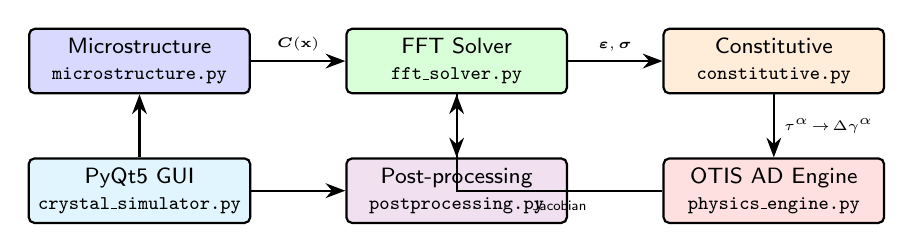
\begin{tikzpicture}[
  box/.style={rectangle, draw, rounded corners=2pt,
              minimum width=2.8cm, minimum height=0.75cm,
              font=\footnotesize, align=center, thick},
  arr/.style={-{Stealth[length=2.5mm]}, thick},
  node distance=0.5cm and 1.2cm
]
  \node[box, fill=blue!15]   (ms)
    {Microstructure\\\texttt{\scriptsize microstructure.py}};
  \node[box, fill=green!15, right=of ms] (fft)
    {FFT Solver\\\texttt{\scriptsize fft\_solver.py}};
  \node[box, fill=orange!15, right=of fft] (cp)
    {Constitutive\\\texttt{\scriptsize constitutive.py}};
  \node[box, fill=red!12, below=0.8cm of cp] (otis)
    {OTIS AD Engine\\\texttt{\scriptsize physics\_engine.py}};
  \node[box, fill=violet!12, below=0.8cm of fft] (pp)
    {Post-processing\\\texttt{\scriptsize postprocessing.py}};
  \node[box, fill=cyan!12, below=0.8cm of ms] (gui)
    {PyQt5 GUI\\\texttt{\scriptsize crystal\_simulator.py}};

  \draw[arr] (ms)  -- (fft)
    node[midway,above,font=\tiny] {$\tens{C}(\bvec{x})$};
  \draw[arr] (fft) -- (cp)
    node[midway,above,font=\tiny] {$\tens\varepsilon,\tens\sigma$};
  \draw[arr] (cp)  -- (otis)
    node[midway,right,font=\tiny] {$\tau^\alpha\!\to\!\Delta\gamma^\alpha$};
  \draw[arr] (otis.west) -| (fft.south)
    node[near start,below,font=\tiny] {Jacobian};
  \draw[arr] (fft) -- (pp);
  \draw[arr] (gui) -- (ms);
  \draw[arr] (gui.east) -- (pp.west);
\end{tikzpicture}
\end{center}

\vspace{0.3em}
\begin{itemize}\setlength\itemsep{2pt}\small
  \item Pure \textbf{NumPy/SciPy} --- no Fortran dependencies.
  \item FFT via \texttt{numpy.fft}
        (drop-in \texttt{pyFFTW} replacement for speed).
  \item Full $(3{\times}3)$ tensor arithmetic avoids
        Voigt-notation pitfalls.
\end{itemize}
\end{frame}

% ----------- Slide 17 -------------------------------------------------------
\begin{frame}{Boundary Conditions and 3D Visualization}
\justifying

The GUI provides \textbf{stress-controlled} input with clear loading visualization:

\vspace{0.3em}
\begin{columns}[T]
\begin{column}{0.48\textwidth}
\textbf{Boundary stress input:}
\begin{itemize}\setlength\itemsep{2pt}\small
  \item Full symmetric stress tensor $\Sbar$ in MPa
  \item Presets: uniaxial, biaxial, hydrostatic, pure shear
  \item Each preset describes \emph{which faces} receive traction
\end{itemize}

\vspace{0.3em}
\textbf{3D preview:}
\begin{itemize}\setlength\itemsep{2pt}\small
  \item Wireframe RVE cube
  \item Traction arrows on each face
  \item \textcolor{red}{Red} $=$ tension,
        \textcolor{blue}{blue} $=$ compression
\end{itemize}
\end{column}
\begin{column}{0.48\textwidth}
\textbf{Result visualization:}
\begin{itemize}\setlength\itemsep{2pt}\small
  \item \textbf{3D}: Von Mises stress on grain
        boundaries with loading arrows overlaid
  \item \textbf{2D slices}: $\sigma_\text{VM}$, $\sigma_{11}$,
        $\varepsilon_{11}$, hydrostatic pressure, grain map
  \item Reports achieved $\avg{\tens\sigma}$ and
        resulting $\avg{\tens\varepsilon}$
\end{itemize}
\end{column}
\end{columns}
\end{frame}

% ----------- Slide 18 -------------------------------------------------------
\begin{frame}{Key Implementation Details}
\justifying

\begin{columns}[T]
\begin{column}{0.48\textwidth}
\textbf{1.\;Tensor-based Green's operator:}
\begin{itemize}\setlength\itemsep{1pt}\small
  \item Fields stored as $(N,N,N,3,3)$
  \item $\bvec{A}^{-1}(\bvec{n})$ pre-computed
        $\to$ $(N,N,N,3,3)$
  \item 9 component-wise FFTs per field
\end{itemize}

\vspace{0.4em}
\textbf{2.\;Periodic Voronoi via KD-tree:}
\begin{itemize}\setlength\itemsep{1pt}\small
  \item Seeds replicated to $3^3{=}27$ images
  \item Query cost: $\mathcal{O}(N^3\log N_g)$
\end{itemize}
\end{column}
\begin{column}{0.48\textwidth}
\textbf{3.\;Convergence criteria:}
\begin{itemize}\setlength\itemsep{1pt}\small
  \item Basic scheme: relative strain change\\
        $\|\tens\varepsilon^{(n+1)}{-}\tens\varepsilon^{(n)}\|
         /\|\tens\varepsilon^{(n)}\|$
  \item CG: residual norm $\|\bvec{r}\|/\|\bvec{b}\|$
  \item Stress control: $\|\Delta\Sbar\|/\|\Sbar\|$
\end{itemize}

\vspace{0.4em}
\textbf{4.\;Spectral equilibrium}
(diagnostic):\\
{\small $\|\xi_j\hat\sigma_{ij}\|/\|\hat\sigma\|$
has ${\sim}7\%$ floor at sharp grain boundaries
--- this is a discretization artifact, not a convergence failure.}
\end{column}
\end{columns}
\end{frame}

% ----------- Slide 19 -------------------------------------------------------
\begin{frame}{Validation and Results}
\justifying

\textbf{1.\;Homogeneous medium} ($\tens{C}=\text{const}$):
error $=0$ in one iteration.\;\checkmark

\vspace{0.3em}
\textbf{2.\;Polycrystalline copper}
($C_{11}{=}168.4$, $C_{12}{=}121.4$, $C_{44}{=}75.4$ GPa):

\begin{center}\small
\begin{tabular}{lcccc}
\toprule
\textbf{Test} & \textbf{Grid}
  & \textbf{$E_\text{eff}$ (GPa)} & \textbf{CG iters} & \textbf{Control} \\
\midrule
8 grains   & $16^3$ & $\approx 202$ & 11 & strain \\
4 grains   & $8^3$  & ---           & 8/Newton & stress \\
\bottomrule
\end{tabular}
\end{center}

\vspace{0.2em}
\textbf{Bounds:}
$E_R = 133$ GPa (Reuss) $< E_H \approx 171$ (Hill)
$< E_\text{FFT} \approx 200$
$< E_V = 210$ GPa (Voigt).\;\checkmark

\vspace{0.3em}
\textbf{3.\;Stress-controlled test} ($\sigma_{11}=500$ MPa, Cu $8^3$):\\
4 Newton iters, $\avg{\sigma_{11}}=500.0$ MPa,
$\avg{\varepsilon_{11}}=0.33\%$.\;\checkmark

\vspace{0.2em}
\textbf{Stress heterogeneity:}
VM stress range $\approx 500$--$1500$ MPa (factor ${\sim}3\times$)
under 1\% uniaxial strain.
\end{frame}

% ----------- Slide 20 -------------------------------------------------------
\begin{frame}{Scalability and Future Work}
\justifying

\begin{columns}[T]
\begin{column}{0.48\textwidth}
\textbf{Current capabilities:}
\begin{itemize}\setlength\itemsep{2pt}\small
  \item Elastic and EVPFFT simulations
  \item Strain- and stress-controlled loading
  \item Arbitrary grains on $N^3$ grids
  \item Interactive PyQt5 GUI with 3D views
  \item 3D boundary stress visualization
\end{itemize}
\end{column}
\begin{column}{0.48\textwidth}
\textbf{Planned extensions:}
\begin{itemize}\setlength\itemsep{2pt}\small
  \item $64^3$--$128^3$ grids
        (\texttt{pyFFTW} + r2c transforms)
  \item Finite-strain:
        $\bvec{F}{=}\bvec{F}^e\bvec{F}^p$
  \item Texture evolution tracking
  \item Non-local EVPFFT~\cite{lebensohn2016}
  \item Phase-field: damage \& recrystallization
\end{itemize}
\end{column}
\end{columns}
\end{frame}

% =============================================================================
%  REFERENCES
% =============================================================================
\begin{frame}[allowframebreaks]{References}
  \bibliography{reference}
\end{frame}

\end{document}
